\chapter{Search}

\section{Search Problems}

Searching is one of the most \itblue{fundemental techniques} in AI, underlying sub-module in many AI systems. Ai can \itblue{solve} many problems that homansare not good at, and achieve \itblue{super-human performance} in many domains (e.g. chess, go, etc.).

\begin{listu}
    \item \textbf{Benefits}

    \begin{listu}
        \item Useful as ageneral algorithmic technique for solving problems, both in AI and in other areas.

        \item Outperform humans in some areas (e.g. games). 

        \item Practical:

        \begin{listu}
            \item Many problems don't have specific algorithms for solving them.
            \item Useful in approximation (e.g., local search in optimization problems).
        \end{listu}

        \item Some critical aspects of intelligent behaviour, e.g., planning, can be cast as search.
    \end{listu}
    
    \item \textbf{Limitations}
    
    \begin{listu}
        \item Only shows how to solve the problem once we have it correctly formulated.
    \end{listu}
\end{listu}

% TODO: Planning and Scheduling Problems:

\subsection{Formalizing a Problem as a Search Problem}

\begin{listu}
    \item Necessary components
    
    \begin{listo}
        \item \bred{State Space}: A \term{state} is a representation of a \itblue{configuration} of the problem domain. The state space is the \itblue{set of all states} include in our model of the problem. 
        \item \bred{Initial State}: The starting configuration. 
        \item \bred{Goal State}: The configuration one wants to achieve. 
        \item \bred{Actions} (or State Space Transitions): Allowed changed to move from one state to another. 
    \end{listo}

    \item Optional Ingredients 
    
    \begin{listu}
        \item \itblue{Costs}: Representing the cost of moving from state to state. 
        \item \itblue{Heuristics}: Help guide the search process. 
    \end{listu}
\end{listu}

Once a search problem is formalized, there are a number of algorithms one can use to solve it. A \term{solution} is a \itblue{sequence of actions} or moves that can transform the \bred{initial state} into a \bred{goal state}. 

\begin{example}[Romania Travel]
    We want to travel in Romania from Arad to Bucharest as fast as possible. 

    \begin{center}
        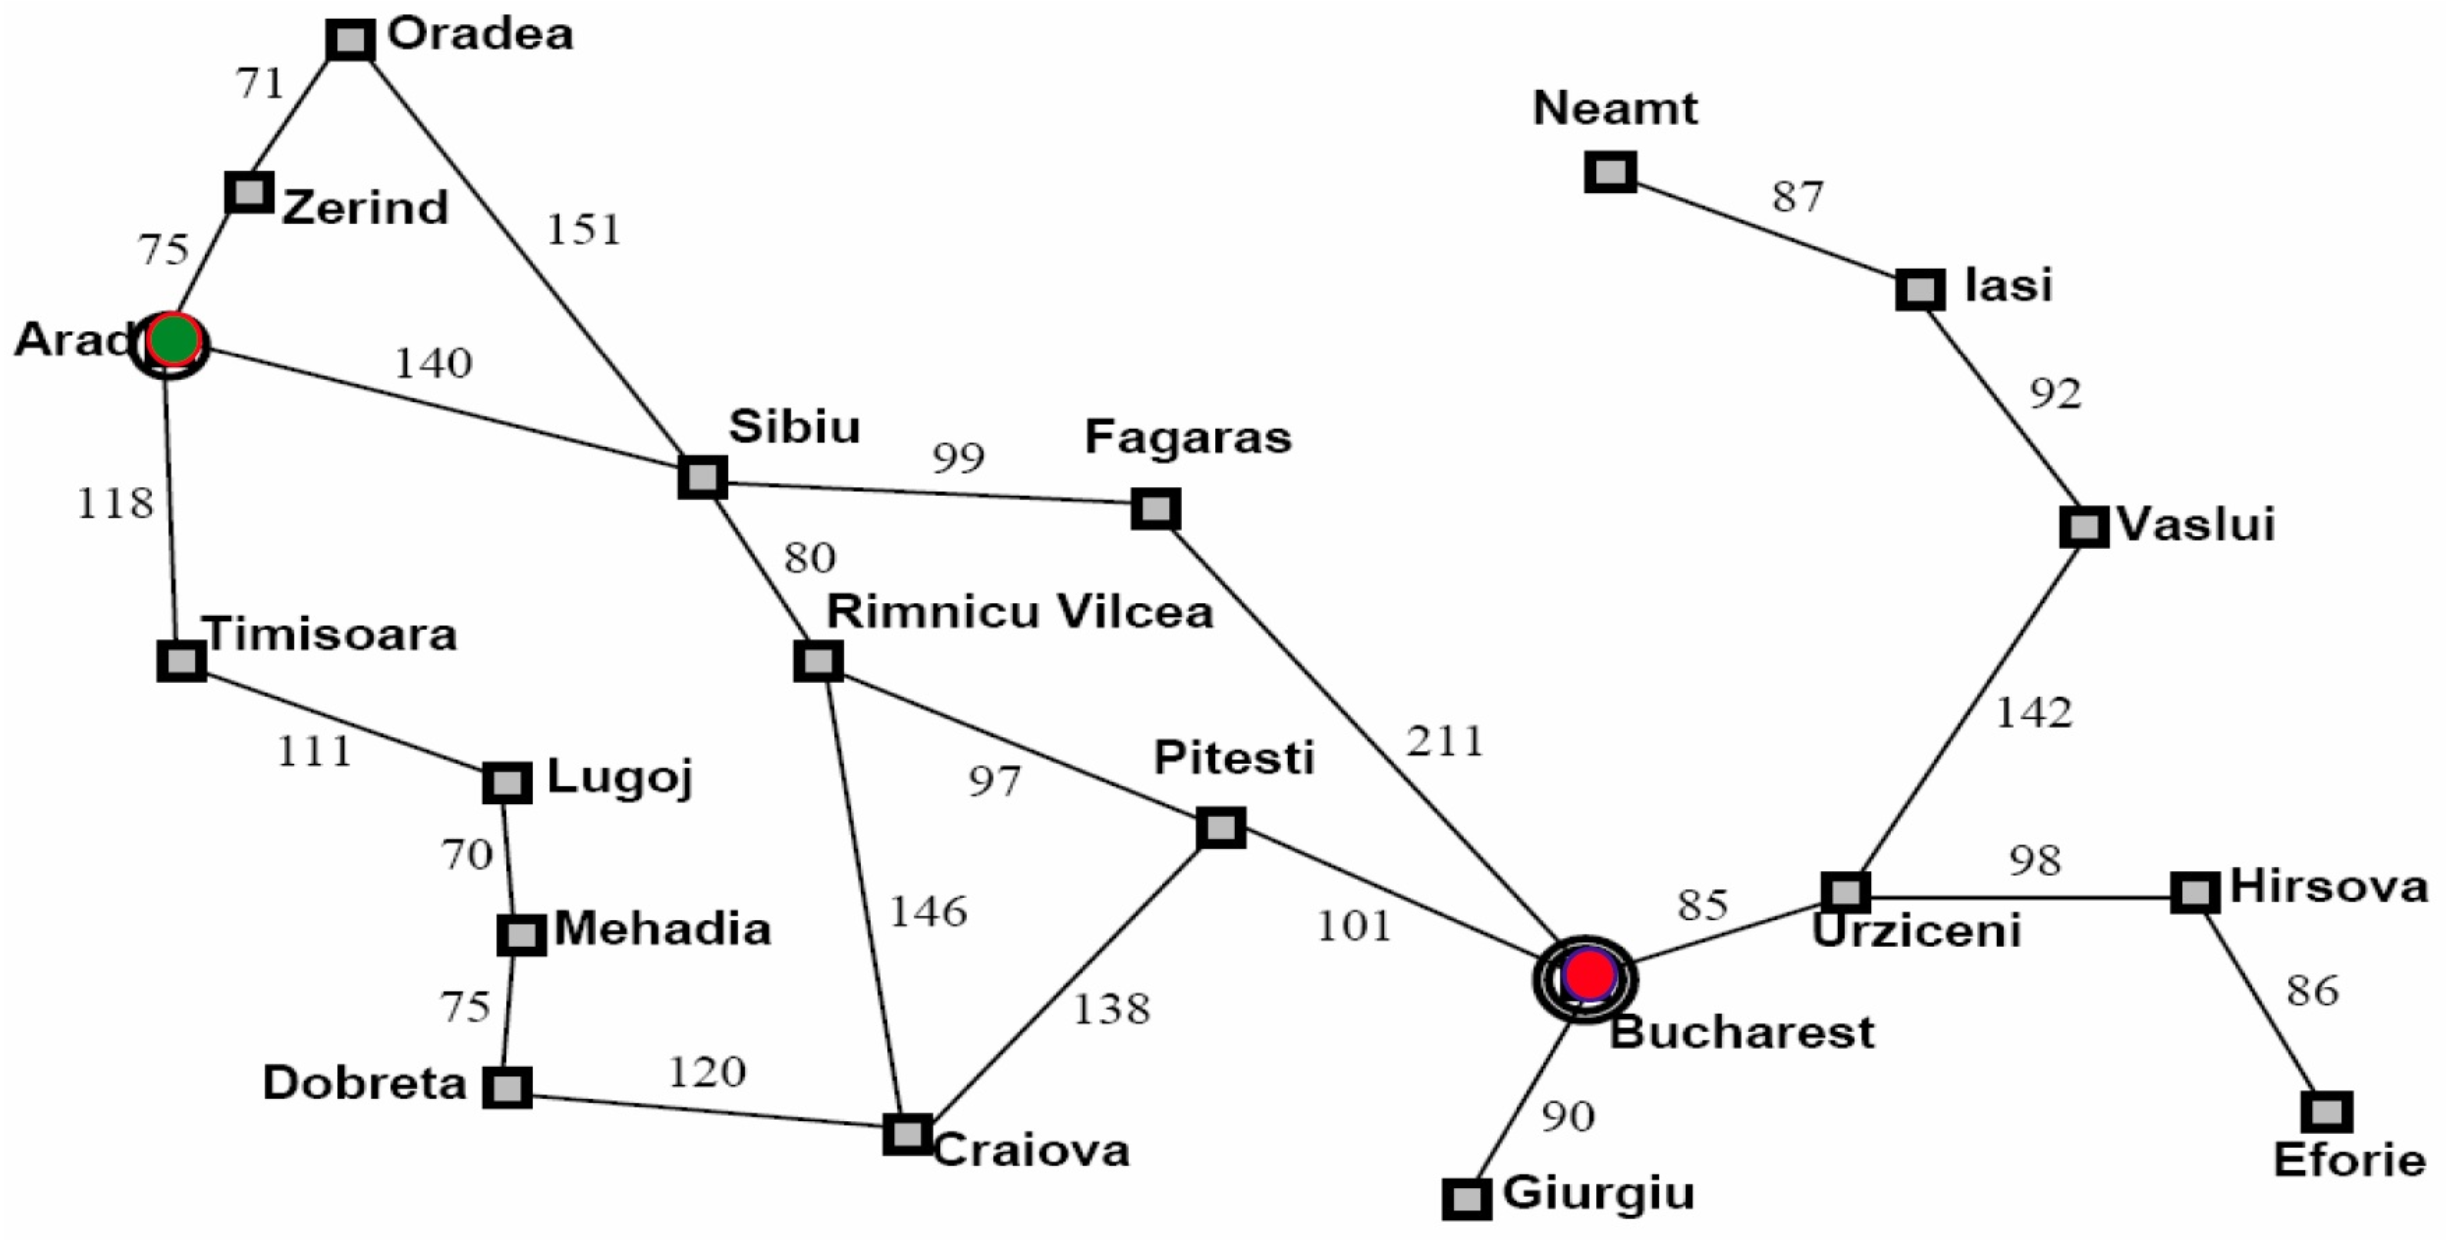
\includegraphics[width=0.75\linewidth]{figures/Romania Travel.png}
    \end{center}

    Each state would be a city. 

    \begin{listu}
        \item \bred{State Space}: The set of all cities on the map.
        \item \bred{Initial State}: Arad.
        \item \bred{Goal State}: Bucharest.
        \item \bred{Actions}: Driving between neighbouring cities.
    \end{listu}
\end{example}

\begin{example}[Water Jugs]
    We have a 3-liter jug and a 4-liter jug. We can fill either jug to the top from a tap, or we can empty either jug onto the ground. We can also pour the contents of one jug into the other until the receiving jug is full or the pouring jug is empty.

    Suppose initially the 4-liter jug is full, we want to have exactly 2 liters in the 3-liter jug.

    {~~~}

    We can use a pair of numbers to represent the state of the system: the amount of water in the 3-liter jug and the amount of water in the 4-liter jug.

    \begin{listu}
        \item \bred{State Space}: The set of all pairs of numbers $(a, b)$ where $a$ is the amount of water in the 3-liter jug and $b$ is the amount of water in the 4-liter jug.
        \item \bred{Initial State}: $(0, 4)$.
        \item \bred{Goal State}: $(2, 0)$, $(2, 1)$, $(2, 2)$, $(2, 3)$, $(2, 4)$.
        \item \bred{Actions}: 
        \begin{listu}
            \item Fill the 3-liter jug from the tap.
            \item Fill the 4-liter jug from the tap.
            \item Empty the 3-liter jug onto the ground.
            \item Empty the 4-liter jug onto the ground.
            \item Pour the contents of the 3-liter jug into the 4-liter jug.
            \item Pour the contents of the 4-liter jug into the 3-liter jug.
        \end{listu}
    \end{listu}

    \begin{remark}
        When formalizing a search problem, always consider these questions:

        \begin{listo}
            \item Can we reach all states fron any given start state?

            \item Will all actions result in a change of state? 

            \bred{No!} Imagine you have $(3, 4)$ and you try to fill the 3-liter jug from the tap. You will still have $(3, 4)$.
        \end{listo}
    \end{remark}
\end{example}

% \subsubsection{More Complex Situations}

In more complex situations, 

\begin{listu}
    \item Actions may lead to \bred{multiple states}. 
    
    For example, filpping a coin may lead to heads or tails.

    \item We may not be \bred{sure of a given state}
    
    For example, when prize is behind door 1, 2, or 3.

    \item Such situations require techniques for reasoning under uncertainty: assign probabilities to given outcomes.
\end{listu}

\subsection{Graphical Representation}

\begin{center}
    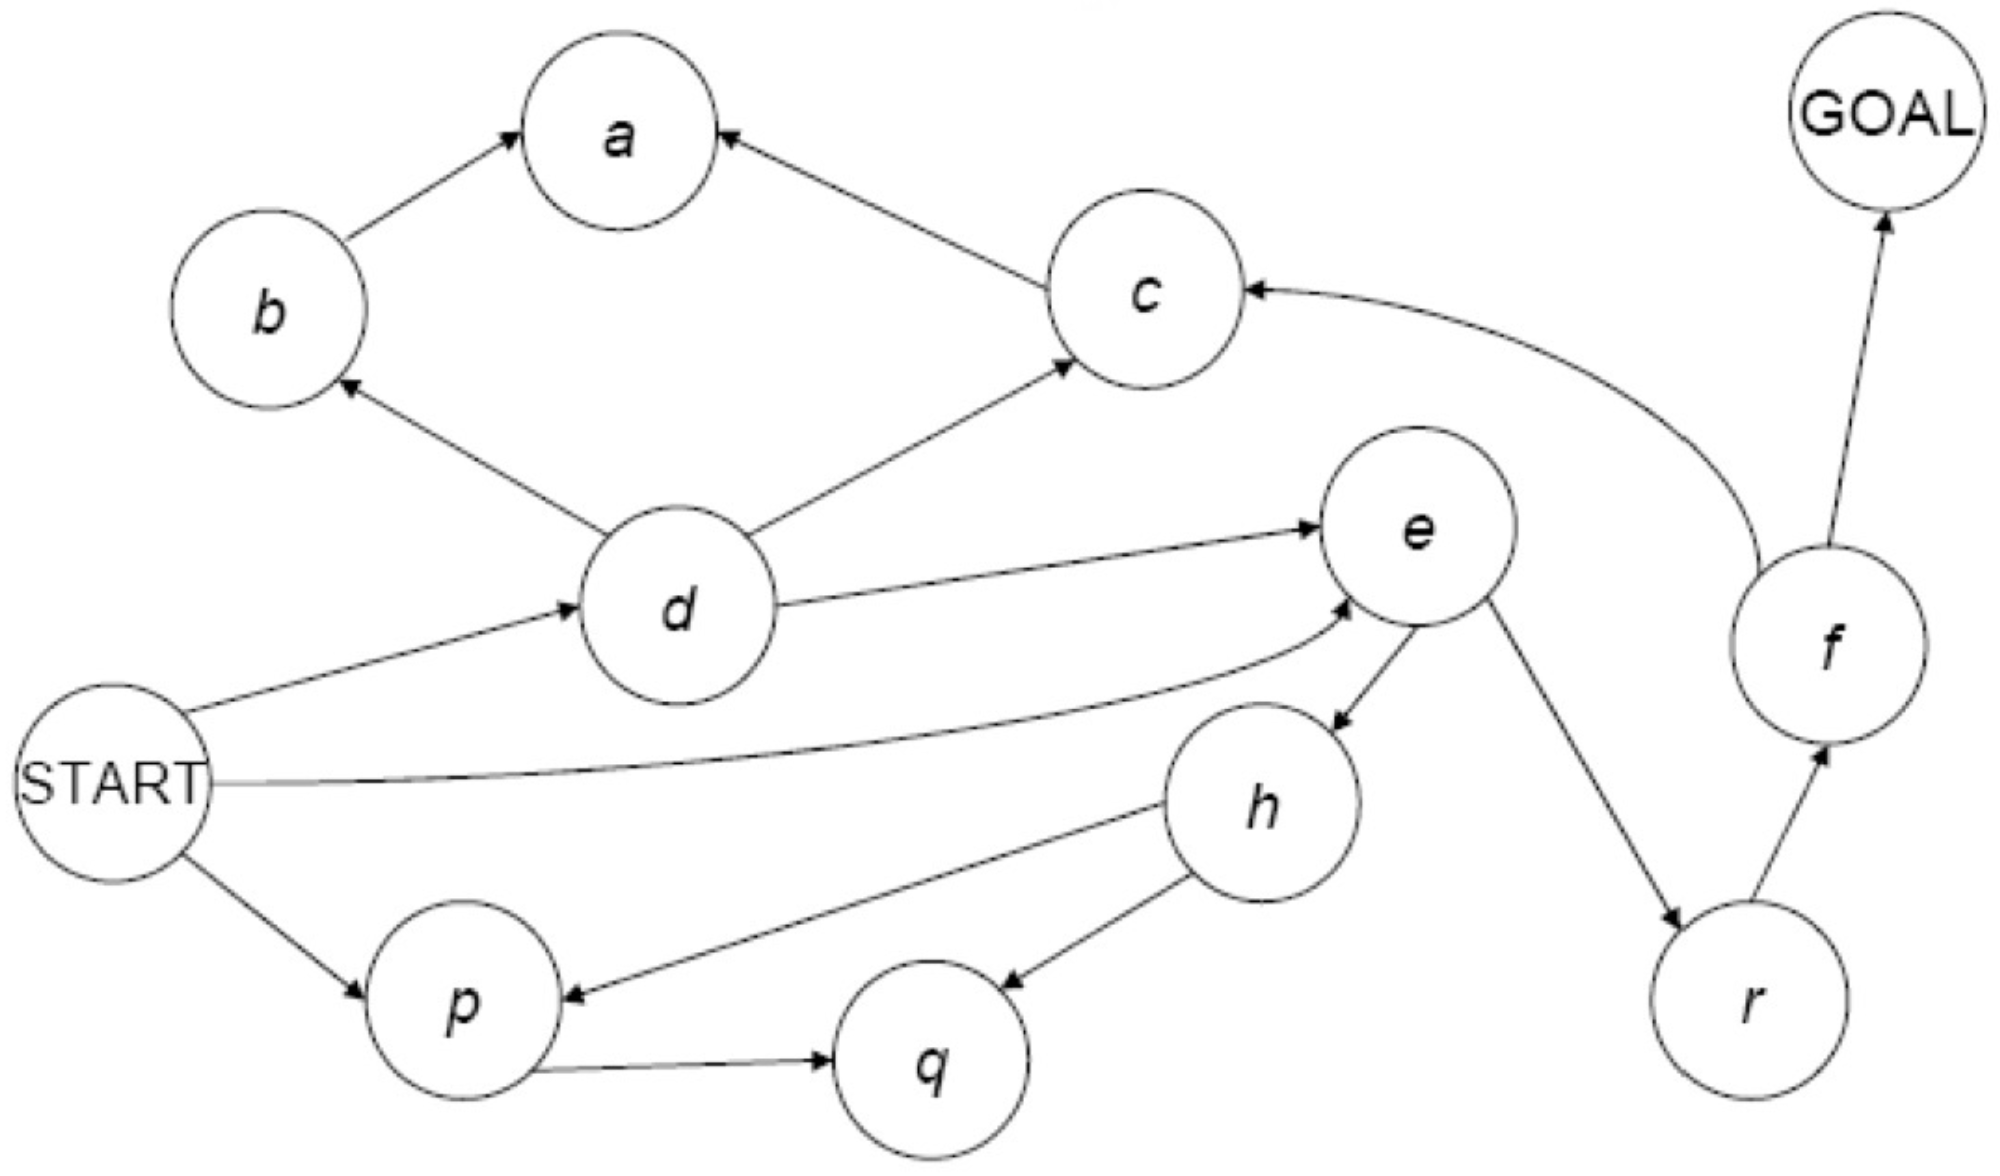
\includegraphics[width=0.5\linewidth]{figures/Search Graph Rep.png}
\end{center}

Assuming a finite search space, the

\begin{listu}
    \item \bred{vertices} represent states in the search space; and the 
    \item \bred{edges} represent transitions resulting from actions (or successor functions).
\end{listu}

\subsubsection{Search Tree}

\begin{definition}[Search Tree]\index{Search Tree}\label{def:search-tree}
    A \term{search tree} is a \itblue{directed graph} where

    \begin{listu}
        \item Each node represents a state.
        \item Each edge represents an action.
        \item The root node represents the initial state.
        \item The leaf nodes represent goal states.
    \end{listu} 
\end{definition}

A search tree reflects the behaviour of an algorithm as it walks through a search problem. It has two important properties:

\begin{listu}
    \item \term{Solution depth}, denoted $d$, the depth of the shallowest goal node in the tree.
    \item \term{Maximum branching factor}, denoted $b$, the maximum number of children of any node in the tree.
\end{listu}

\begin{remark}
    Note that the \bred{same} state may appear \bred{multiple times} in a search tree.
\end{remark}

\begin{remark}
    It is important to distinguish between \bred{states} from \bred{nodes}. 

    \begin{listu}
        \item A \bred{state} represents a possible configuration of the world. 
        \item A \itblue{node} is a data structure constituting part of a search tree. It includes 
        \begin{listu}
            \item a \bred{state} and 
            \item the \bred{parent node}, 
            \item the \bred{action} that led to this node, and 
            \item the \bred{cost} of the path from the initial node to this node. 
        \end{listu}
        \item  Intuitively speaking, each node corresponds with a path from the initial state to the node's state.
        \item Two \bred{different nodes} are allowed to contain the \bred{same world state}.
    \end{listu}
\end{remark}

\subsection{Algorithms for Search}

\begin{listu}
    \item \textbf{Input}
    
    \begin{listu}
        \item \textbf{Initial node}

        \item \textbf{Successor Function} $S(x)$
        
        returns the set of nodes that can be reached from node $c$ via a single action. 

        \item \textbf{Goal Test Function} $G(x)$
        
        returns true if node $c$ satisfies the goal condition. 

        \item \textbf{Action Cost Function} $C(x, a, y)$
        
        returns the cost of moving from node $x$ to node $y$ using action $a$.

        Note that $C(x, a, y) = \infty$ if $y$ is not reachable from $a$ via $a$. 
    \end{listu}

    \item \textbf{Output}
    
    \begin{listu}
        \item A \itblue{sequence of actions} that transforms the initial node satisfying the goal test. 
        \item The sequence might be, \term{optimal in cost} for some algorithms, \term{optimal in length} for some algorithms, come with \bred{no optimality} guarantees from other algorithms.
    \end{listu}

    \item \textbf{Procedure}
    
    \begin{listu}
        \item Put nodes have not yet expanded in a list called the \term{\Frontier} (or \term{Open}).
        \item Initially, only the \itblue{initial node} is in the \Frontier.
        \item At each iteration, pull a node from the \Frontier, apply $S(x)$, and insert the children back into the \Frontier.
        \item Repeat until pulling a goal node.
    \end{listu}
\end{listu}

% \newpage
\begin{algorithm}
    \caption{Tree Search Algorithm}
    
    \begin{algorithmic}[1]
        \Function{Tree-Search}{Frontier, Successors, Goal?}
            % If frontier is empty, return failure
            \If{Frontier is empty}
                \State \Return failure
            \EndIf

            \State Curr $\gets$ select state from frontier

            \If{Goal?(Curr)}
                \State \Return Curr
            \EndIf

            \State \Frontier' $\gets$ (Frontier $-$ \{ Curr \}) $\cup$ Successors(Curr)

            \State \Return \Call{TreeSearch}{Frontier', Successors, Goal?}
        \EndFunction
    \end{algorithmic}
\end{algorithm}

% TODO: example

Note that the search terminates only when a goal node is expanded into the \Frontier.

\subsubsection{Critical Properties of Search}

\begin{listu}
    \item \textbf{Completeness}
    
    \begin{listu}
        \item A search algorithm is \term{complete} if it always finds a solution if one exists.
    \end{listu}

    \item \textbf{Optimality}
    
    \begin{listu}
        \item A search algorithm is \term{optimal} if it always finds a solution with the lowest cost.
    \end{listu}

    \item \textbf{Time Complexity}
    
    \begin{listu}
        \item The \term{time complexity} of a search algorithm is the number of nodes it expands or generates. 
    \end{listu}

    \item \textbf{Space Complexity}
    
    \begin{listu}
        \item The \term{space complexity} of a search algorithm is the maximum number of nodes it stores in memory.
    \end{listu}
\end{listu}

\section{Uninformed Search Algorithms}

\subsection{Uninformed Search Strategies}

The \bred{order} of nodes in the \Frontier determines the behaviour of the search algorithm. It determines whether or not the algorithm is complete, optimal, and how much time and space it requires. Search algorithms differ in their selection rule, but they all keep the \Frontier as an ordered set. The question of which node to select next from the \Frontier is now equivalent to the question of how to order the \Frontier.

There are strategies that adpot a \itblue{fixed-rule} for selecting the next node to be expanded. These strategies are called \term{uninformed search strategies} because they do \bred{not} use any \itblue{domain specific informatioin} about the problem other than the definition of the problem itself. These strategies include Breadth-First Search, Depth-First Search, Uniform-Cost Search, Depth-Limited Search, and Iterative Deepening Search. 

In those course, it is assumed that the graph we are searching is \itblue{explicitly} represented as an adjacency list (or adjacency matrix). However, this will \bred{not} work when there an exponential number of nodes and edges. In AI applications, there are typically an exponential number of nodes, making it impossible to explicitely represent them all. AI search algorithms work with \itblue{implicitly} defined state spaces, where actions are compacted as \itblue{successor state functions}, and nodes must contaion enough information to allow the successor state function to be applied.

\subsection{Breadth-First Search (BFS)}

\begin{definition}[Breadth-First Search]\index{Breadth-First Search}\label{def:bfs}
    \term{Breadth-First Search} is a search strategy that expands the shallowest unexpanded node first.
\end{definition}

BFS explores the search tree \itblue{level by level}. It place the children of the current node at the \bred{end} of the \Frontier. This means the \Frontier is a \itblue{queue}, and we always extract the \itblue{first} element from the \Frontier.

\begin{example}
    We run BFS on the following graph,

    \begin{center}
        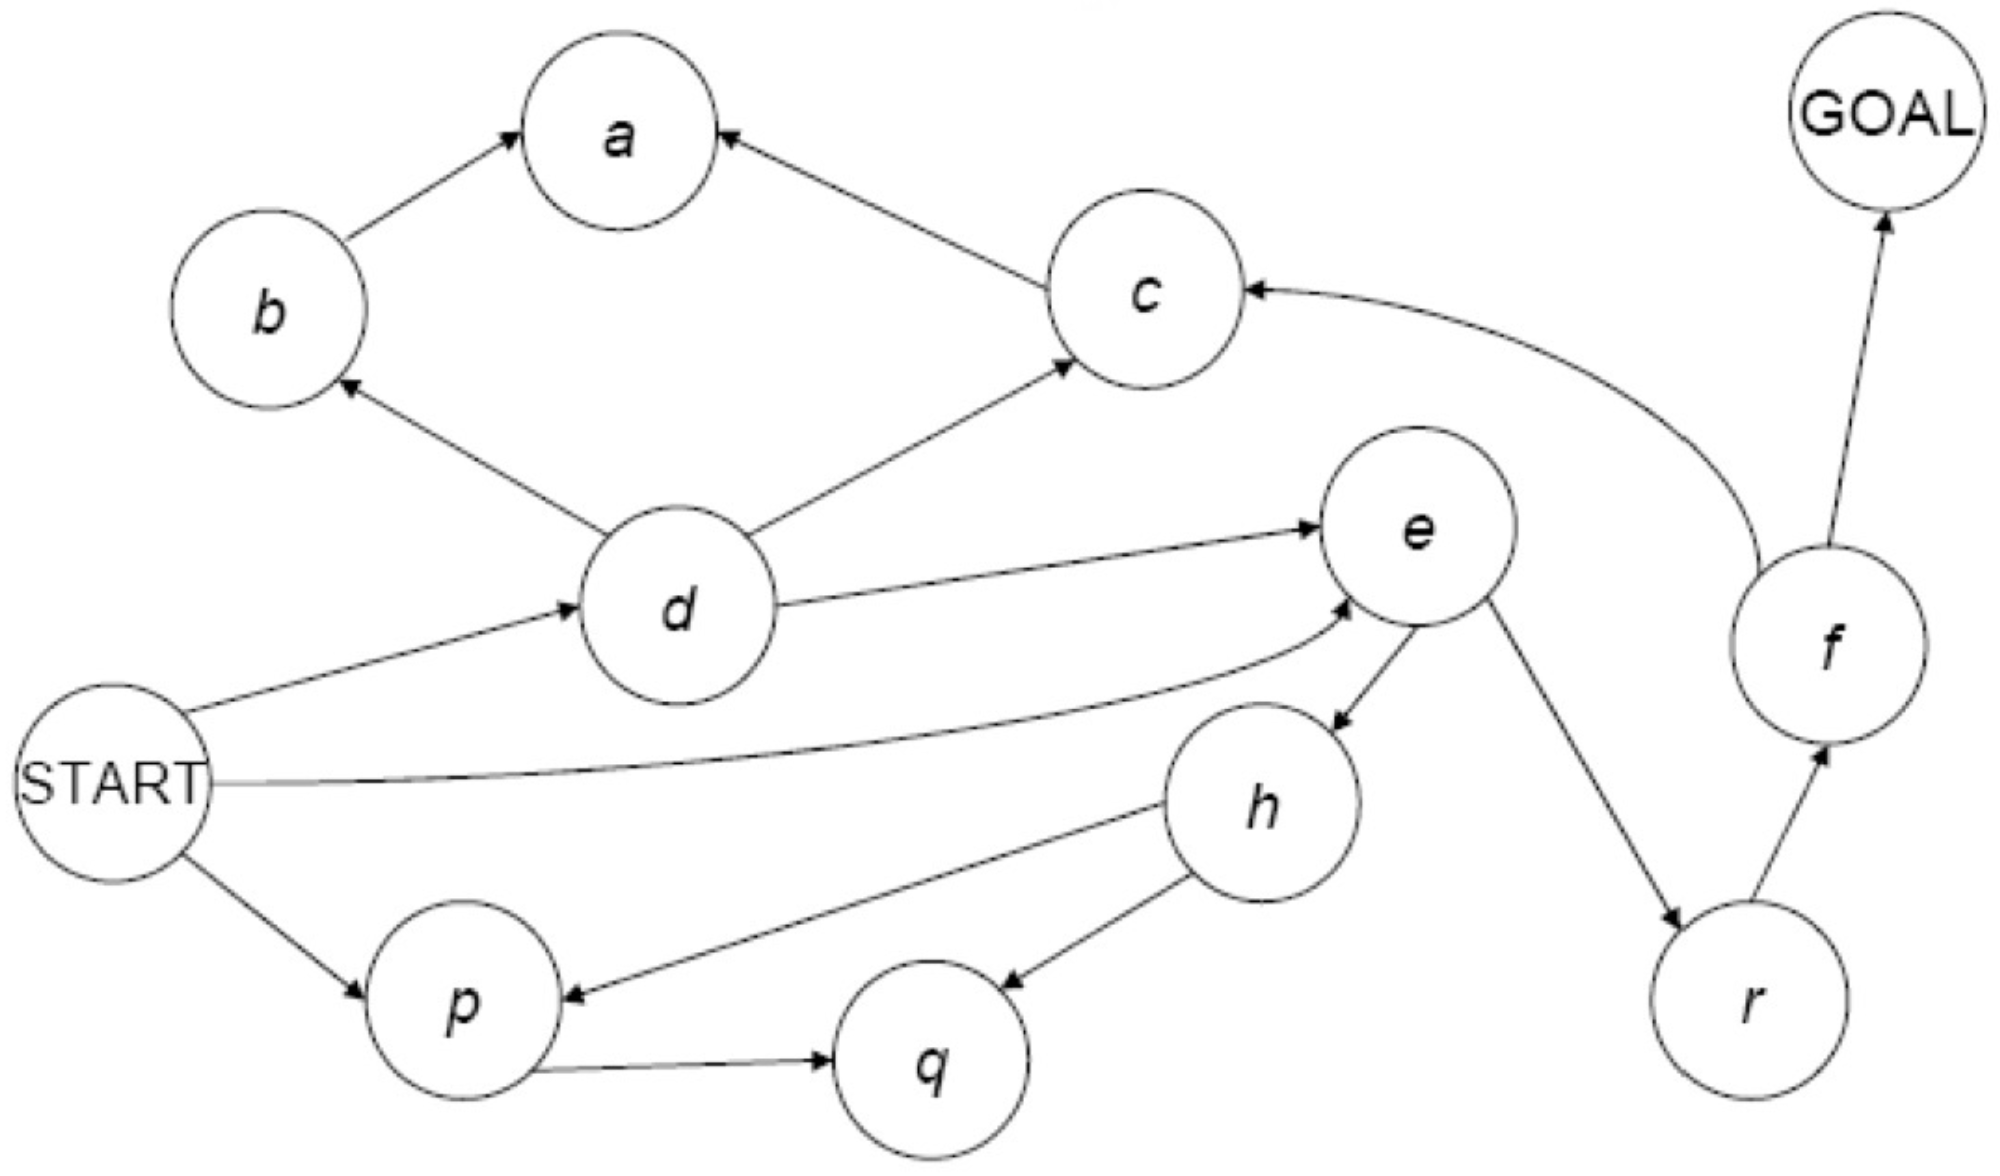
\includegraphics[width=0.45\linewidth]{figures/Search Graph Rep.png}
    \end{center}

    which yields the search tree

    \begin{center}
        \tikzexternalenable
        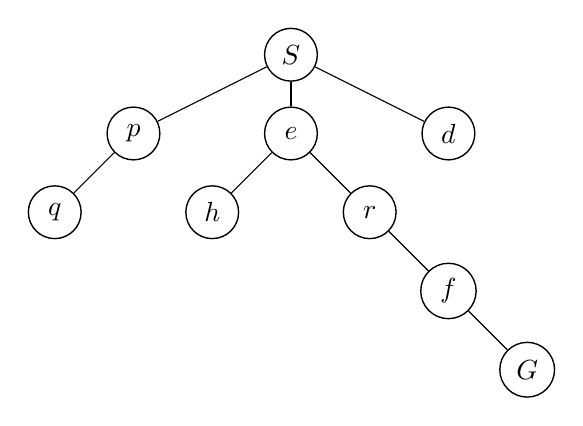
\begin{tikzpicture}[ tree-node/.style={ circle, draw=black, line width=0.5pt, minimum size=0.67cm, } ]
            \node[tree-node] (S) at (0, 0) {$S$};
            \node[tree-node] (P) at (-2, -1) {$p$};
            \node[tree-node] (E) at (0, -1) {$e$};
            \node[tree-node] (D) at (2, -1) {$d$};
            \node[tree-node] (Q) at (-3, -2) {$q$};
            \node[tree-node] (H) at (-1, -2) {$h$};
            \node[tree-node] (R) at (1, -2) {$r$};
            \node[tree-node] (F) at (2, -3) {$f$};
            \node[tree-node] (G) at (3, -4) {$G$};

            % Edges
            \draw (S) -- (P);
            \draw (S) -- (E);
            \draw (S) -- (D);
            \draw (P) -- (Q);
            \draw (E) -- (H);
            \draw (E) -- (R);
            \draw (R) -- (F);
            \draw (F) -- (G);
        \end{tikzpicture}
        \tikzexternaldisable
    \end{center}
\end{example}

\begin{listu}
    \item \textbf{Completeness}
    
    \begin{listu}
        \item BFS is \term{complete} if the \bred{branching factor} is \itblue{finite}.
        \item The length of the path (from the initial node to the node removed from the \Frontier) is \itblue{non-decreasing}, as we replace eac expanded node with path langth $k$ with a node with path length of $k + 1$. 
    \end{listu}

    \item \textbf{Optimality}
    
    \begin{listu}
        \item BFS gives the \bred{shortest length solution}. 

        All nodes with shorter paths are expanded prior to any node with longer path. We examine all paths of length $< k$ before all paths of length $k$. Thus, if there is a solution with length $k$, we will find it before longer solutions. 

        \item BFS is \bred{not optimal} in terms of \itblue{cost}.
        
        BFS does not take into account the cost of the path. It is possible that a longer path has a lower cost than a shorter path.
    \end{listu}
\end{listu}

% TODO: Romnia Travel Example, see slides page 35

\subsubsection{Properties of BFS}

Let $b$ be the maximum branching factor and $d$ be the depth of the shallowest goal node.

\begin{listu}
    \item \textbf{Time Complexity} \[
        1 + b + b^2 + \cdots + b^d + b(b^d - 1) \in O(b^{d+1})
    \]

    The last term id $b(b^d - 1)$ because we need to remove the goal node, who does not need any successors.

    \item \textbf{Space Complexity} \[
        \bigo{b^{d+1}}
    \]
    
    In the worst case, only the last node of depth $d$ satisfies the goal. So all nodes at depth $d$ except the last one will be expanded by the search and each such expansion will add up to $b$ new nodes to the \Frontier.
\end{listu}

\begin{table}[ht!]
    \renewcommand{\arraystretch}{1.25}
    \centering
    \begin{tabular}{| l | l | l | l |}
        \hline
        Depth & Paths    & Time          & Memory    \\ \hline
        1     & $1$      & 0.01 millisec & 100 bytes \\ \hline
        6     & $10^6$   & 10 sec.       & 100 MB    \\ \hline
        8     & $10^8$   & 17 min.       & 10 GB     \\ \hline
        9     & $10^{9}$ & 3 hrs.        & 100 GB    \\ \hline
    \end{tabular}
\end{table}

Space complexity is a bigger problem than time complexity. Typically, BFS rus out of memory before it runs out of time.

\subsection{Depth-First Search (DFS)}

\begin{definition}[Depth-First Search]\index{Depth-First Search}\label{def:dfs}
    \term{Depth-First Search} is a search strategy that expands the deepest unexpanded node first.
\end{definition}

DFS explores the search tree \itblue{branch by branch}. It place the children of the current node at the \bred{front} of the \Frontier. This means the \Frontier is a \bred{stack}, and we always extract the \itblue{first} element from the \Frontier.

\begin{example}
    We run DFS on the following graph,

    \begin{center}
        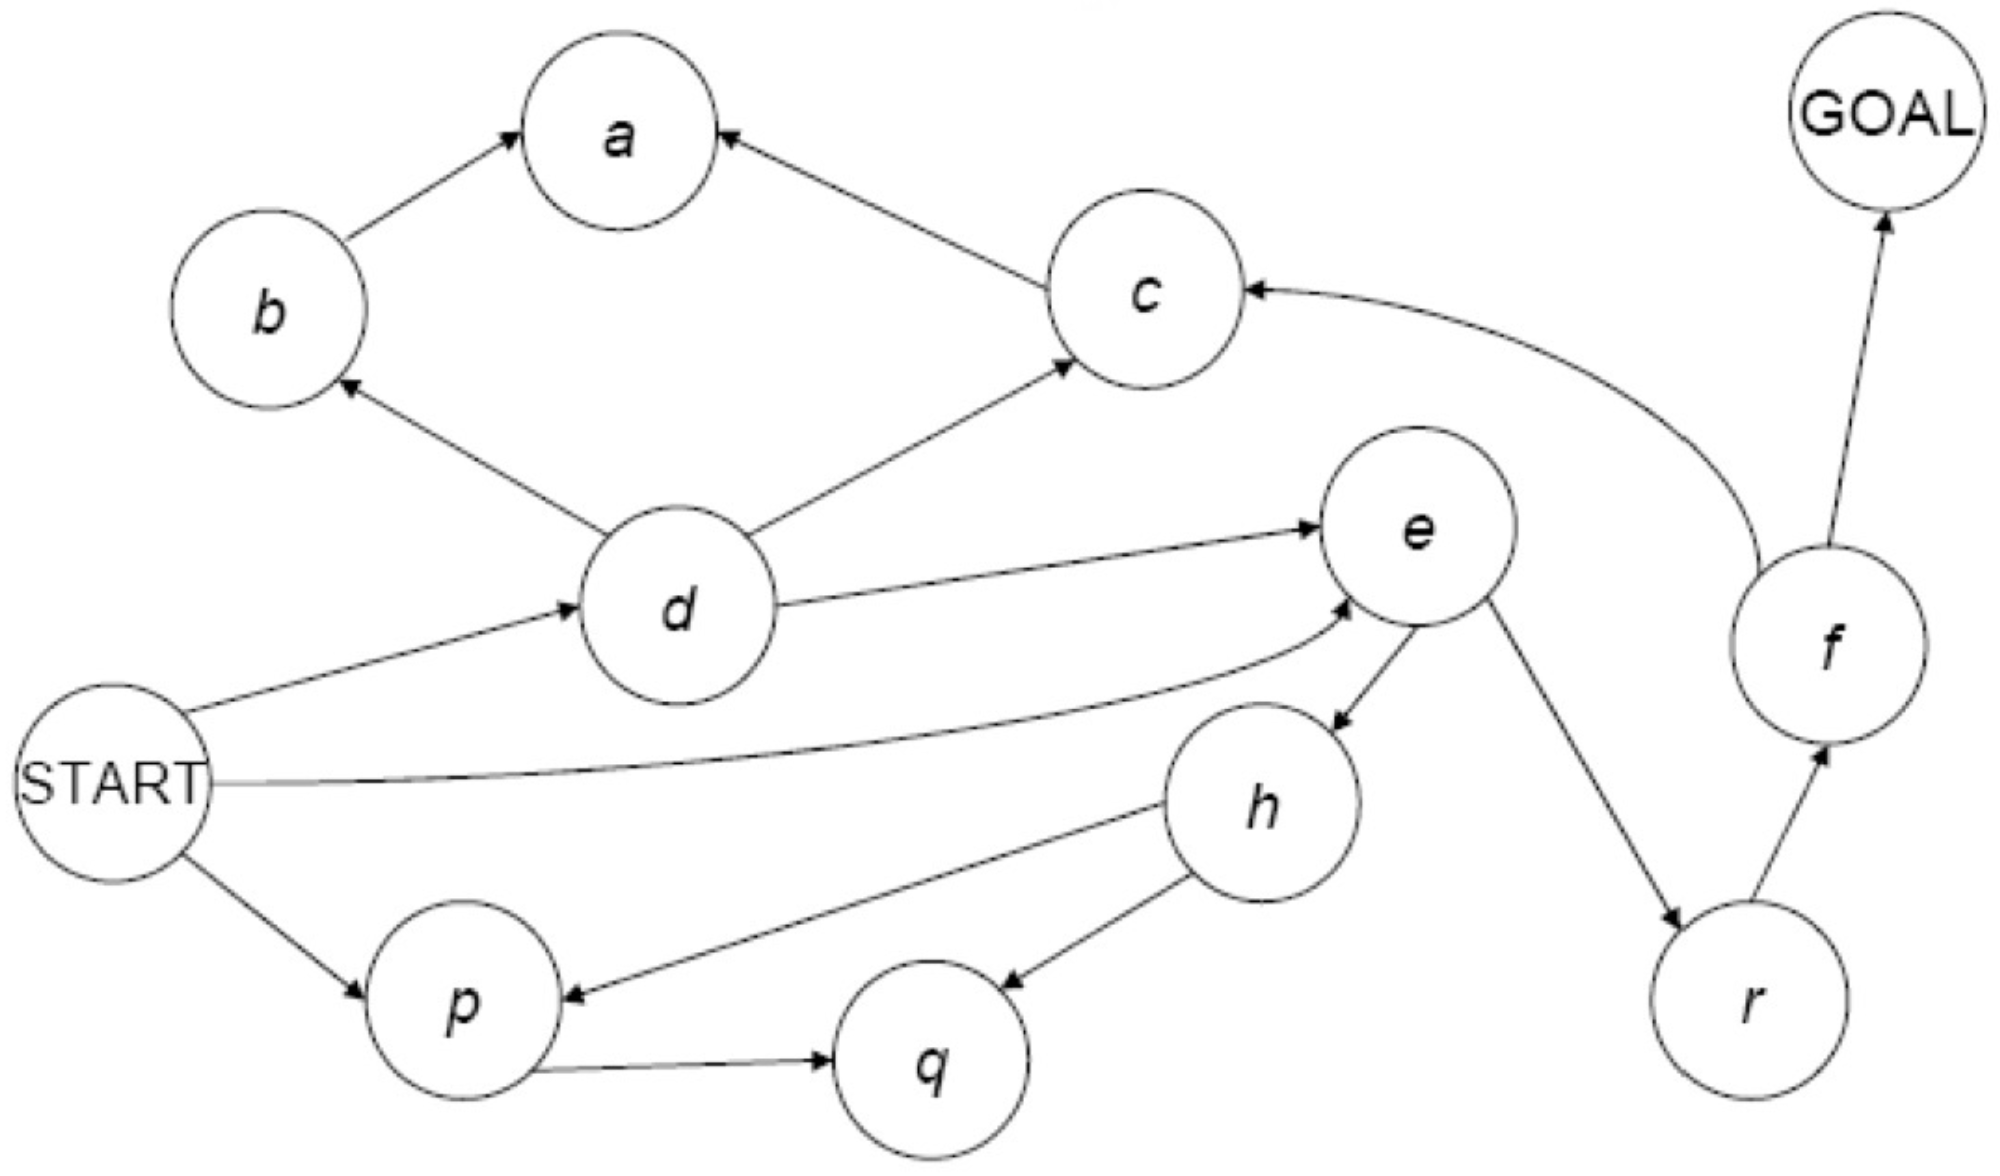
\includegraphics[width=0.45\linewidth]{figures/Search Graph Rep.png}
    \end{center}

    The \Frontier changes as follows:

    \begin{center}
        \begin{tabular}{| c | c | c |}
            \hline
            \textbf{Frontier} & \textbf{Node Removed} & \textbf{Successors Added} \\ \hline \hline
            $S$               & $S$                   & $d, e, p$                 \\ \hline
            $d, e, p$         & $d$                   & $b, c, e$                 \\ \hline
            $b, c, e, e, p$   & $b$                   & $a$                       \\ \hline
            $a, c, e, e, p$   & $a$                   & $\null$                   \\ \hline
            $c, e, e, p$      & $c$                   & $a$                       \\ \hline
            $a, e, e, p$      & $a$                   & $\null$                   \\ \hline
            $e, e, p$         & $e$                   & $h, r$                    \\ \hline
        \end{tabular}

        {~~~}

        $\cdots$
    \end{center}
\end{example}

\begin{listu}
    \item \textbf{Completeness}
    
    \begin{listu}
        \item DFS is \term{not complete}. \bred{Infinite} paths cause incompleteness.
        \item This is because DFS does not keep track of visited nodes, so it can get stuck in a loop. An infinite search space can also cause DFS to run forever.
        \item We can prune paths with \bred{cycles} to get completeness, if state space is finite. 
    \end{listu}

    \item \textbf{Optimality}
    
    \begin{listu}
        \item DFS is \term{not optimal} in terms of \itblue{length} or \itblue{cost}.
        \item DFS returns the \itblue{first} solution it finds, which may not be the \itblue{shortest} or \itblue{cheapest} solution.
    \end{listu}
\end{listu}

\subsubsection{Properties of DFS}

Let $b$ be the maximum branching factor and $m$ be the maximum depth of the search tree.

\begin{listu}
    \item \textbf{Time Complexity} \[
        \bigo{b^m}
    \] where $m$ is the length of the \itblue{longest path} in the state space.

    \begin{listu}
        \item This is \bred{very bad} if $m$ is much larger than $d$, but if there are \itblue{mant solution paths}, DFS may be much faster than BFS.
        \item Using \term{Heuristics}, we can determine which successor to explore first. 
    \end{listu}

    \item \textbf{Space Complexity} \[
        \bigo{bm}
    \]
    
    DFS has a \bred{linear} space complexity, which is a significant advantage. 

    This is because DFA only explores a single branch of the search tree at a time. \Frontier only contains the current node $v$ along with the $m$ descendants of $v$.  Each node can have at most $b$ unexplored siblings and there are at most $m$ nodes on the current branch, which gives $\bigo{bm}$.
\end{listu}

\subsection{Depth-Limited Search (DLS)}

Despite DFS being \itblue{incomplete} and \itblue{non-optimal}, it has a great advantage over BFS: \itblue{linear space complexity}. This makes it possible to use DFS in situations where BFS would run out of memory. 

In order to address the incompleteness of DFS, we can impose a \itblue{depth limit} $D$ on the search. This means that we will only explore paths of length $D$ or less. If we reach a node at depth $D$ that is not a goal node, we will \itblue{backtrack} and explore other paths. This is called \term{Depth-Limited Search} (DLS).

\begin{definition}[Depth-Limited Search]\index{Depth-Limited Search}\label{def:dls}
    \term{Depth-Limited Search} is a search strategy that expands the deepest unexpanded node first, but only up to a given depth limit $D$.
\end{definition}

\begin{listu}
    \item {\color{darkGreen}\textbf{Benefit}:} DLS overcomes the infinite length paths issue, 
    \item \bred{Limitation:} DLS only finds a solution if the \itblue{depth limit} $D$ is greater than or equal to the depth of the shallowest goal node $d$. 
\end{listu}

\begin{remark}
    The root of a search tree is at depth 0. A path consisting onlty of the root node has length 0.

    Recall that the length of a path is the number of actions (edges) in the path. 
\end{remark}

\begin{center}
    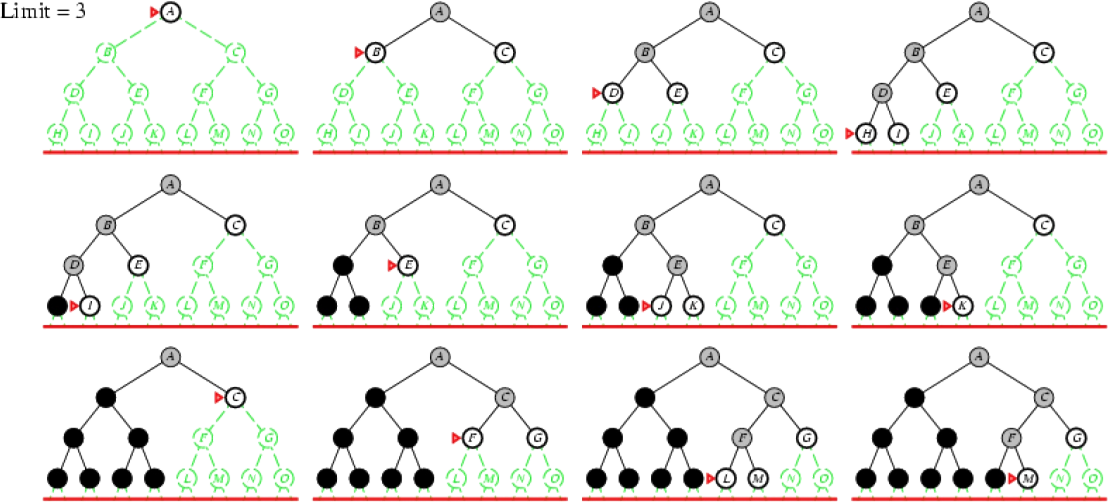
\includegraphics[width=0.67\linewidth]{figures/ids-limit-3.png}
\end{center}

\begin{algorithm}[ht!]
    \caption{Depth-Limited Search Algorithm}
    \begin{algorithmic}[1]
        \Function{DLS}{start, frontier, successors, goal?, maxd}
            \State frontier.insert(<start>)
            \Comment{frontier must be a stack for DFS}
            \State cutoff $\gets$ false
            \While{frontier is not empty}
                \State curr $\gets$ frontier.extract()
                \Comment{Remove node from frontier}
                \If{goal?(curr.final())}
                    \State \Return curr, cutoff 
                    \Comment{curr is solution}
                \ElsIf{\Call{Length}{curr} $<$ maxd}
                \Comment{Only successors if lendth(curr) < maxd}
                    \For{succ $\in$ successors(curr.final())}
                        \State frontier.insert(<p, succ>)
                    \EndFor
                \Else
                    \State cutoff $\gets$ true
                    \Comment{Reached depth limit, some nodes not expanded}
                \EndIf
            \EndWhile

            \State \Return failure, cutoff
        \EndFunction
    \end{algorithmic}
\end{algorithm}

\subsection{Iterative Deepening Search (IDS)}

DLS is \itblue{complete} if the \itblue{depth limit} $D$ is greater than or equal to the depth of the shallowest goal node $d$. However, we do not know $d$ in advance. We can start at a depth limit $D = 0$, and iteratively \bred{increase} $D$ until we find a solution. We stop if {\color{darkGreen}\textbf{a solution is found}}, or the search \bred{failed without cutting off} any nodes because of the depth limit. This is called \term{Iterative Deepening Search} (IDS).

Note that if no nodes were cut off, the search examined all nodes in the state space and found nosolution, hence there is no solution. 

\begin{definition}[Iterative Deepening Search]\index{Iterative Deepening Search}\label{def:ids}
    \term{Iterative Deepening Search} is a search strategy that repeatedly applies DLS with increasing depth limits until a solution is found.
\end{definition}

\begin{center}
    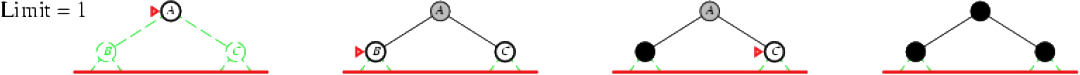
\includegraphics[width=0.67\linewidth]{figures/ids-limit-1.png}
    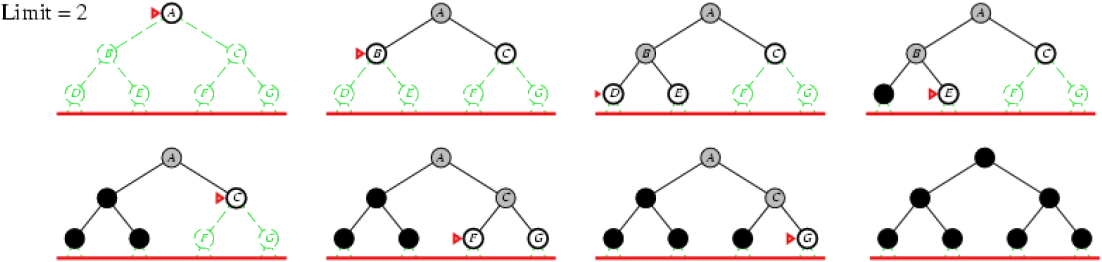
\includegraphics[width=0.67\linewidth]{figures/ids-limit-2.png}
    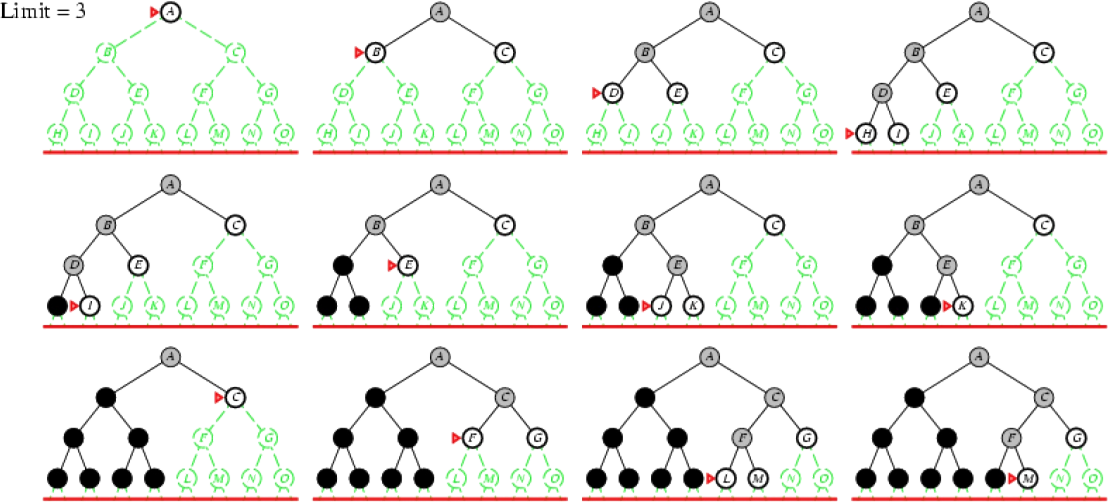
\includegraphics[width=0.67\linewidth]{figures/ids-limit-3.png}
\end{center}

\begin{algorithm}[ht!]
    \caption{Iterative Deepening Search Algorithm}

    \begin{algorithmic}
        \Function{IDS}{start, frontier, successors, goal?}
            \State depth $\gets$ 0
            \While{true}
                \State solution, cutoff $\gets$ \Call{DLS}{start, successors, goal?, depth}
                \If{solution is not failure}
                    \State \Return solution
                \ElsIf{cutoff is false}
                \Comment{No nodes at deeper levels exist, no solution}
                    \State \Return failure
                \EndIf
                \State depth $\gets$ depth + 1
            \EndWhile
        \EndFunction
    \end{algorithmic}
\end{algorithm}

\begin{listu}
    \item \textbf{Completeness}
    
    \begin{listu}
        \item IDS is \term{complete}. 
    \end{listu}

    \item \textbf{Optimality}
    
    \begin{listu}
        \item IDS gives the \bred{shortest length solution}.

        \item IDS is \term{not optimal} in terms of \itblue{cost}, for the same reason as DFS.
        
        We can make IDS optimal by doing the following:

        \begin{listu}
            \item Can use a \bred{cost bound} instead of depth bound.
            \item Only expand nodes of cost \itblue{less} than the cost bound. 
            \item Keep track of the \term{minimum cost unexpanded node} in each iteration, \itblue{increase the cost bound} to that on the next iteration.
            \item Can be \bred{computationally expensive} since need as many iterations of the search as there are distinct node costs.
        \end{listu}
    \end{listu}
\end{listu}

\subsubsection{Properties of IDS}

\begin{listu}
    \item \textbf{Time Complexity} \[
        (d+1)b^0 + db^1 + (d-1)b^2 + \cdots + b^d \in \bigo{b^d}
    \]

    \begin{listu}
        \item This is \bred{very bad} if $d$ is much larger than $m$, but if there are \itblue{mant solution paths}, IDS may be much faster than BFS.
        \item Using \term{Heuristics}, we can determine which successor to explore first. 
    \end{listu}

    \item \textbf{Space Complexity} \[
        \bigo{bd}
    \]
    
    The space complexity of IDS is still linear. 
\end{listu}

\begin{remark}
    Comparing to BFS, 

    \begin{itemize}
        \item The {\color{darkGreen}time complexity} of IDS can be better since it does not expand nodes at the solution depth, while BFS (in the worst case) must expand all the \itblue{bottom later nodes} until it expands a goal node. However, with a simple optimization BFS can achieve the \itblue{same time complexity} as IDS.

        \item The {\color{darkGreen}space complexity} of IDS is much better.
        \begin{listu}
            \item In practice, BFS can be buch better depending on the problem: effective \bred{cycle checking} can be employed with BFS
            \item IDS cycle checking will make the space complexity as bad as BFS. 
        \end{listu}
    \end{itemize}
\end{remark}

\subsection{Path Checking and Cycle Checking}

\subsubsection{Path Checking}

\begin{definition}[Path Checking]\index{Path Checking}\label{def:path-checking}
    \term{Path Checking} is a search strategy that checks whether a node is an ancestor of itself along the path from the initial node to the node.
\end{definition}

\begin{remark}[Notation]
    \begin{listu}
        \item A path $p_k$ is represented as a typle of states $\langle s_0, s_1, \cdots, s_k \rangle$ where $s_0, s_1, \cdots, s_k$ are states in $p_k$ in the order they appear in the path.
        \item Suppose $s_k$ is expanded to obtain a child succcessor statce $c$. The obtained path $\langle s_0, s_1, \cdots, s_k, c \rangle$ can be written as $\langle p_k, c \rangle$.
    \end{listu}
\end{remark}

\begin{listu}
    \item In every path $\langle p_k, c \rangle$ where $p_k$ is the path $\langle s_0, s_1, \cdots, s_k \rangle$, ensure that the \bred{final state} $c$ is not equal to any ancestors of $c$ along this path. That is, \[
        c \notin \{ s_0, s_1, \cdots, s_k \}
    \]

    \item Paths are checked in \bred{isolation}
    
    \item {\color{darkGreen}\textbf{Benefit}:} Does not increase time and space commplexity. 
    
    \item \bred{Limitation}: Does not prune all the redundant states. 
\end{listu}

\begin{example}
    Consider the Romania Travel problem. Below is an example of a search tree. 

    \begin{center}
        % \tikzexternalenable
        % \begin{tikzpicture}
        %     % Elipse node, black stroke, white background, text `Arad' in node
        %     \node[draw, circle, fill=white] (Arad) at (0, 0) {Arad};

        % \end{tikzpicture}
        % \tikzexternaldisable
        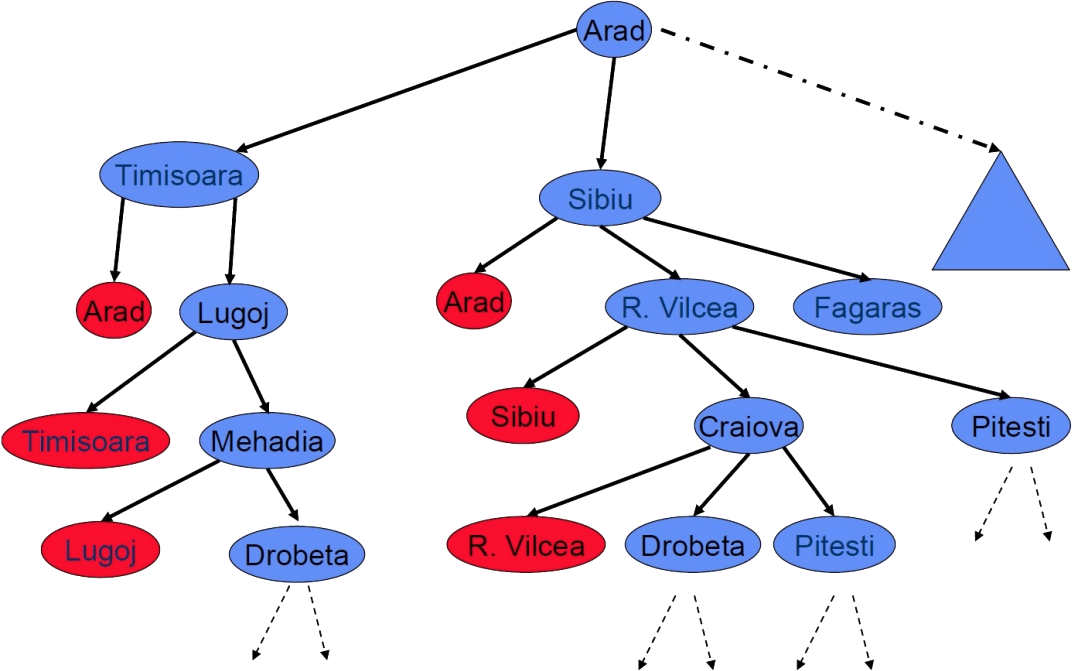
\includegraphics[width=0.67\linewidth]{figures/path-checking.png}
    \end{center}

    The nodes coloured in red are pruned by path checking, as they are ancestors of the current node.
\end{example}

\subsubsection{Cycle Checking}

Cycle checking is also called \term{Multiple path checking}. It is a \itblue{more general} version of path checking. It checks whether a node has been expanded before, not just whether it is an ancestor of itself along the path from the initial node to the node. 

\begin{definition}[Cycle Checking]\index{Cycle Checking}\label{def:cycle-checking}
    \term{Cycle Checking} is a search strategy that checks whether a node has been expanded before.
\end{definition}

\begin{listu}
    \item Keep track of \bred{all} nodes previous expanded during the search using a list called the \term{closed list}.
    
    \item When we expand $n_k$ to obtain successor $c$, 
    
    \begin{listu}
        \item Ensure that $c$ is not equal to any \itblue{previously expanded} node.
        \item If it is, we \bred{do not add} $c$ to the \Frontier. 
    \end{listu}

    \item {\color{darkGreen}\textbf{Benefit}:} Very \itblue{effective} in pruning redundant states.
    
    \item \bred{Limitation}: Expensive in term of \bred{space}. 
    
    The space complexity is $\bigo{b^{d}}$ with optimization, and $\bigo{b^{d+1}}$ without optimization (which is the same as BFS).
\end{listu}

\begin{remark}
    We cannot utilize this technique with DFS. This is because DFS only puts a node in the closed list after all its descendants have been expanded. Thus, the ``root'' node will be put on the list later than its descendants, and cycle checking will fail.

    Moreover, the space complexity of DFS with cycle checking would be exponential, which will loose the advantage of DFS.
\end{remark}

\begin{example}
    Consider the Romania Travel problem. Below is an example of a search tree. 

    \begin{center}
        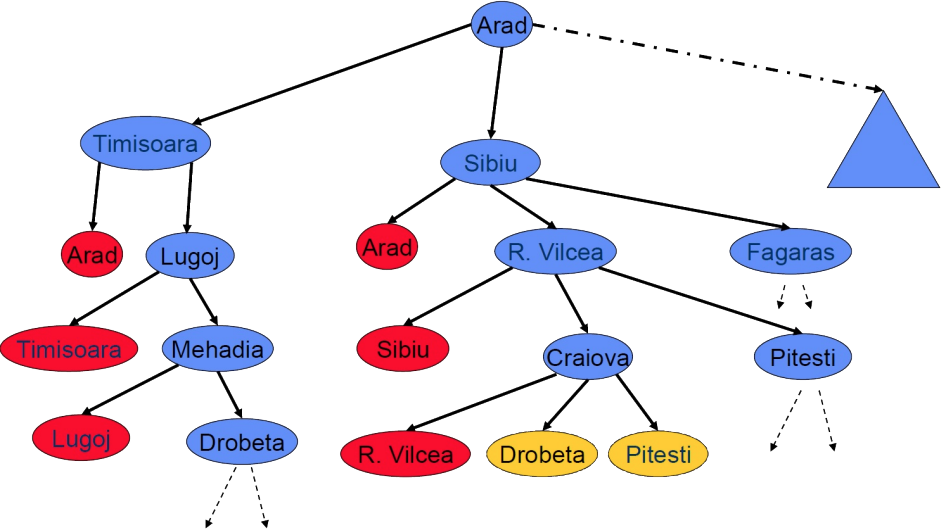
\includegraphics[width=0.67\linewidth]{figures/cycle-checking.png}
    \end{center}

    The nodes coloured in red are the explored ancestors, and the nodes coloured yellow are the nodes already exploare in another branch.
\end{example}

\subsubsection{Optimal Cost}

If we reject a path $\langle p, c \rangle$ because we have previously seen state $c$ via a different path $p'$, it could be that $\langle p, c \rangle$ is a cheaper path to $c$ than $p$

The solution would be keeping track of each state as well as the \bred{known minimum cost} of a path to that state. 

\begin{listu}
    \item If a more \bred{expensive} path to a previously seen state is found, do not add the corresponding node to the \Frontier.
    \item If a cheaper path to a previously seen state is found, add the corresponding node to the \Frontier and
    \begin{listu}
        \item \itblue{Remove} other more \itblue{expensive} nodes to the same state from the \Frontier, OR
        \item Lazily, \itblue{ignore} these more expensive nodes when/if they are removed for expansion.
    \end{listu}
\end{listu}

\subsection{Uniform-Cost Search (UCS)}

The \term{Uniform-Cost Search} (UCS) algorithm is a variant of BFS that uses \itblue{cost} as the criterion for selecting the next node to expand. UCS expands the node with the \itblue{lowest path cost} $g(n)$, where $g(n)$ is the cost of the path from the initial node to node $n$.

\begin{definition}[Uniform-Cost Search]\index{Uniform-Cost Search}\label{def:ucs}
    \term{Uniform-Cost Search} is a search strategy that expands the node with the lowest path cost $g(n)$.
\end{definition}

\begin{remark}
    UCS is a \itblue{generalization} of BFS. BFS is UCS with a \itblue{constant cost} of 1 for each action.
\end{remark}

\begin{center}
    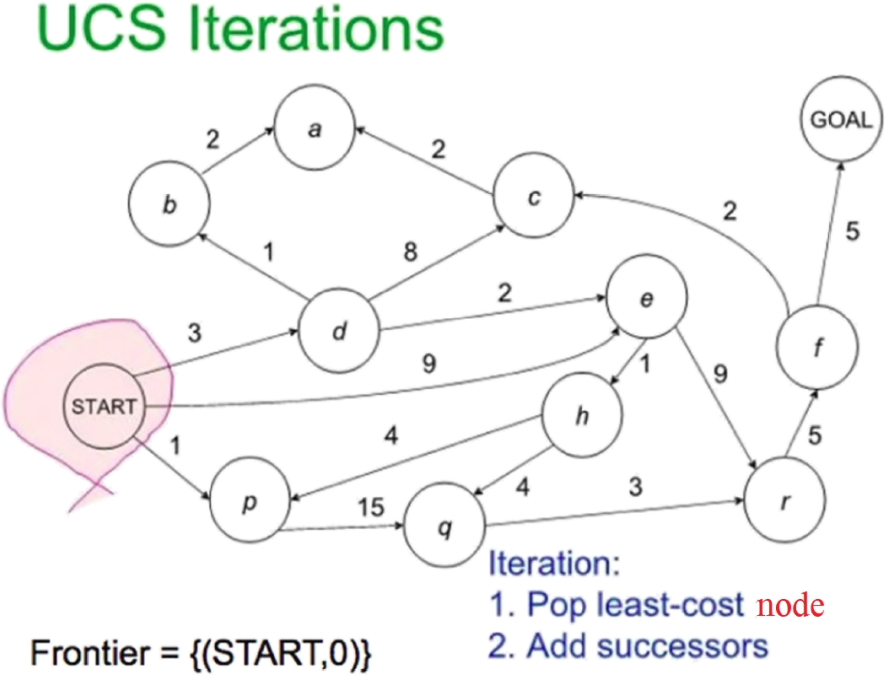
\includegraphics[width=0.45\linewidth]{figures/ucs-1.png}
    \hfill
    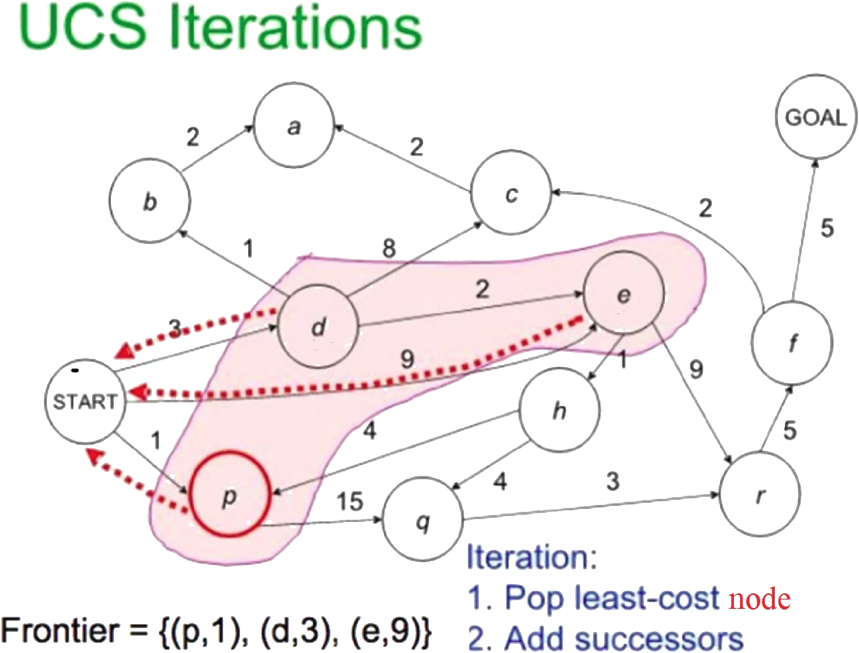
\includegraphics[width=0.45\linewidth]{figures/ucs-2.png}

    {~~~}

    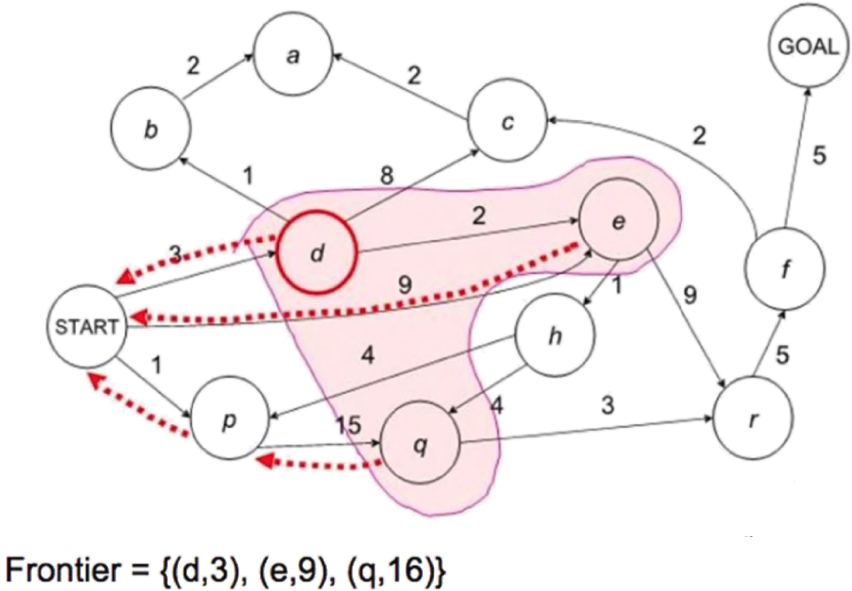
\includegraphics[width=0.45\linewidth]{figures/ucs-3.png}
    \hfill
    $\dots$
\end{center}

\begin{listu}
    \item \textbf{Completeness}
    
    \begin{listu}
        \item UCS is complete under the condition that there is a \bred{non-zero constant lower-bound $\epsilon$} on the cost of every action.

        That is, each transition from one state to another must have a cost of at least $\epsilon > 0$.

        \item Under  this condition the cost of the nodes chosen to be expanded will be non-decreasing and eventually we will expand all nodes with cost equal to the cost of a solution path
    \end{listu}

    \item \textbf{Optimality}
    
    \begin{listu}
        \item UCS finds the \bred{minimum cost} solution if each transition has cost $\ge \epsilon > 0$.
        
        \item UCS explores nodes in the search space in non-decreasing order of cost. So it must find minimum cost path to a goal before finding any higher costs paths leading to a goal.
    \end{listu}

    \begin{proof}
        UCS is optimal if the cost of each action is $\ge \epsilon > 0$.

        \begin{remark}[Intuition]
            \begin{listu}
                \item nodes are expanded in order of \bred{non-decreasing cost}.
                \item \bred{All nodes} with cost strictly less than $C$ are expanded before \bred{all nodes} with cost equal to $C$.
                \item The first path found to a state is the \bred{cheapest} path to that state (be it a goal state or not).
            \end{listu}
        \end{remark}

        In all of the following lemmas the assumption is that each transition has cost $\ge \epsilon > 0$.

        \begin{lemma}
            Let $c(n)$ denote the cost of a node n on the \Frontier. If a node $n_2$ is expanded after $n_1$ by UCS, then $\color{darkRed}c(n_1) \le c(n_2)$.
        \end{lemma}

        \begin{lemma}
            Let $n$ be an arbitrart node expanded by UCS in a search tree. All the nodes in the search space with cost strictly less than $c(n)$ are expanded \bred{before $n$}.
        \end{lemma}

        \begin{lemma}
            Let $p$ be the first path UCS find whose final state is a state $s$. Then $p$ is a \bred{minimal cost} path to $s$.
        \end{lemma}
    \end{proof}
\end{listu}

\subsubsection{Properties of UCS}

The time and space complexity of UCS are both \[
    \bigo{ b^{\floor{C^* / \epsilon} + 1} }
\]

\begin{listu}
    \item UCS has to expand \itblue{all nodes} with cost \bred{less} than $C^*$ and potentially \itblue{all nodes} with cost \bred{equal} to $C^*$. 
    \item In the worst case, there are $\bigo{ b^{\floor{C^* / \epsilon} + 1} }$ nodes with cost \itblue{less than or equal to} $C^*$. 
\end{listu}

\begin{remark}
    in the worst case, there are $\color{darkRed} \floor{C^* / \epsilon}$ actions on the optimal path, and each state has $b$ successors, where $C^*$ denotes the cost of the optimal solution path. We also assume each action has cost $\ge \epsilon > 0$.
\end{remark}